\section{Staatsfinanzen \ho{Ho11-12}}
\subsection{Instrumente der Geldpolitik \ho{Ho11 F9}}
  Der Staat kommt durch Steuern zu Geld. Das f�hrt aber zu einem
  Wohlfahrtsverlust. Man sollte bei unelastischen Kurven steuern erheben, also
  m�glichst nicht bei Luxusg�tern!
    \begin{multicols}{2}
	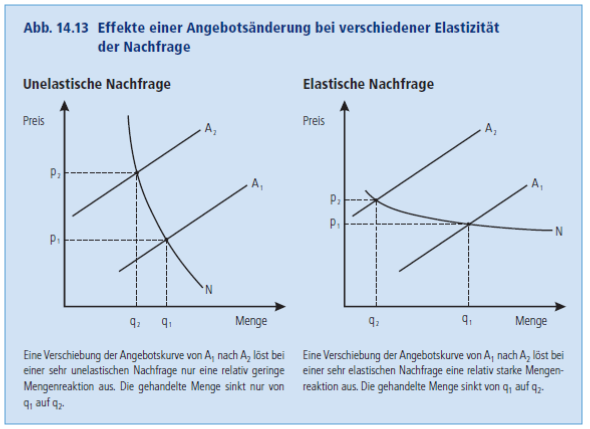
\includegraphics[width=9cm]{./bilder/h11f09.png} \\
	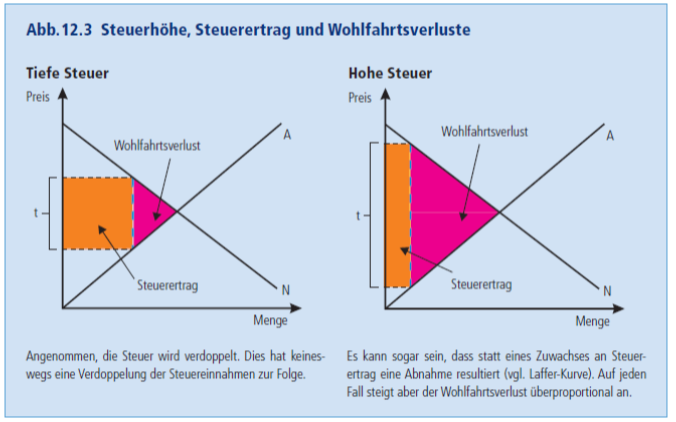
\includegraphics[width=9cm]{./bilder/h11f14.png} \\
	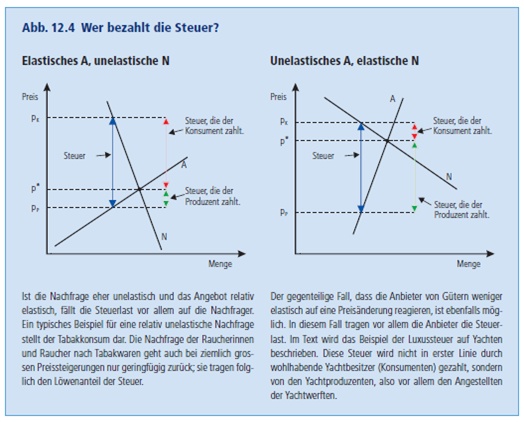
\includegraphics[width=9cm]{./bilder/h11f16.png} \\
	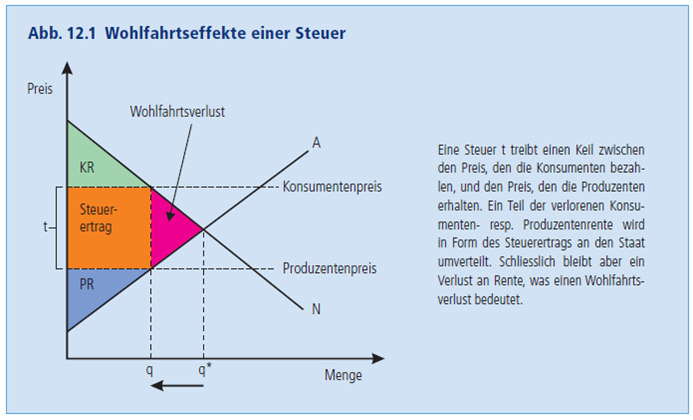
\includegraphics[width=9cm]{./bilder/h11f07.png} 
\end{multicols}

\subsection{Schuldenbremse}
  Verschuldet sich der Staat muss er die Schulden in den kommenden Jahren
  komplett wieder abbauen. Das sorgt f�r eine kontrollierte Verschuldung. Die
  USA setzen ihr Schuldenbremsen-Limit einfach immer h�her anstatt die Schulden
  abzubauen.\\
  Die USA verloren ihre AAA Wertung weil sie die Limite nicht gen�gend schnell
  erh�ht haben. Ihnen wird also nicht mehr zugetraut in Zukunft diesen
  politischen Entscheid innert Frist zu f�llen.
